\documentclass[10pt,english]{article}
\usepackage{geometry}
 \geometry{verbose,tmargin=2cm,bmargin=2cm,footskip=1cm}
\usepackage{babel}
\usepackage{bm}
\usepackage{amssymb}
\usepackage{amsmath}
\usepackage{multirow}
\usepackage{graphicx}
\usepackage{setspace}
\usepackage{enumitem}
\onehalfspacing


\def\vss{\vspace{1cm}}
\def\vs{\vspace{0.2cm}}

\begin{document}

\noindent
\centerline{
\textbf{\large Numerical Methods for the Solution of Differential Equations (AM 213B)}}\\
\centerline{{\bf Homework 4 - grading form}}
%
\centerline{\line(1,0){480}}\vspace{.cm}

\vspace{0.2cm}
\flushleft{\bf Name:} Dante Buhl
\vs
\flushleft{\bf Final score:} write your final score here, for instance, 93/100.

\vss\noindent
\centerline{\bf Point allocation explanation}


\vs
{\bf Question 1 (20/20 points):} 
\begin{enumerate}[label=\alph*)]
    \item The same result is obtained in the work (that is consistent with order 1 in time and
    order 2 in space). The result shown is obtained using taylor expansions
    however the exact expansions used are not explicitly shown except after
    substitution. 
    \item Using the Von Neumann Stability theory, the same result is obtained
    which shows the eigenvalues of $\boldsymbol{G}$ being less than 1 in
    absolute magnitude. 

\end{enumerate}

\vs   
{\bf Question 2 (30/30 points):} 
\begin{enumerate}[label=\alph*)]
    \item Student successfully proves through two bouts of integration that the
    value of the integral is conserved in time. 
    \item Plots obtained are identical except for the variation in plotting
    method. (Mine just shows the contour lines where Daniele's shows a filled in
    plot)
\end{enumerate}

\vs
{\bf Question 3 (50/50 points):} 
\begin{enumerate}[label=\alph*)]
    \item Plots are similar with an exeptiopn of what seems to be small errors
    present in Daniele's finite difference scheme. Mine is slightly different
    and enforces periodicity in the differentiation matrix rather than overly in
    the timestepping scheme. Thus I am able to get a plot which looks better and
    only used N gridpoints (as opposed to N+2 as assignment instructed).
    \item Plot of the integral value of the finite difference scheme behaves as
    expected and remains constant at 1. 
    \item The maximum pointwise error plot while having slightly different
    magnitudes of error has the same general trend in time. 
    \item Though I claimed that the scheme's mean squared error decayed
    quadratically, after doing some more analysis on the plotted line, it seems
    that the decay is closer to order 3 or order 4. This is obtained by actually
    fitting a slope to the line in log-log space. This is futher abetted by the
    fact that the error decay in Daniele's plot seems to be steeper than an
    order 2 convergence suggesting that his plot is actually order 3 or 4 as
    well. 
    Note that I forgot to produce a log log plot on my actual assignment, so
    I've attached a log log plot of the same data here. (See Figure 1). 
    \begin{figure}
        \centering
        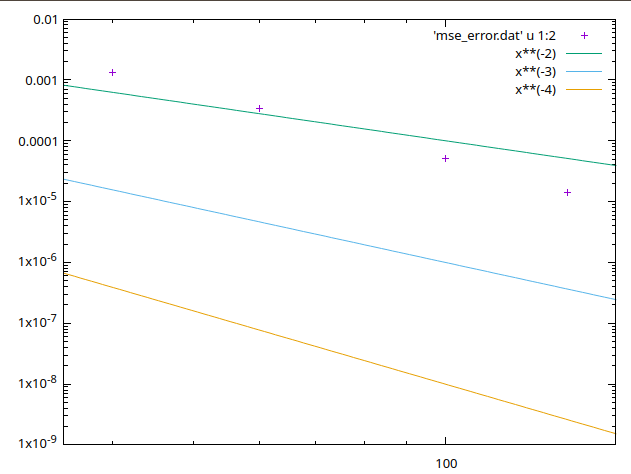
\includegraphics[width=.7\textwidth]{mse_updated.png}
        \caption{Updated MSE on a log-log plot with order 2, 3, and 4
        convergence for comparison.}
    \end{figure}
\end{enumerate}


\end{document}
